% !TEX spellcheck = en_US

\documentclass[conference]{IEEEtran}
\usepackage{cite}
\usepackage{amsmath,amssymb,amsfonts}
\usepackage{algorithmic}
\usepackage{graphicx}
\usepackage{textcomp}
\usepackage{xcolor}
% add hyperlinks, delete all .aux files if adding hyperref after previous build
\usepackage{hyperref}
% support for unicode charcters like "é" and "ñ"
\usepackage[T1]{fontenc}
% Provides generic commands \degree, \celsius, \perthousand, \micro and \ohm
\usepackage{gensymb}
% splits a section into multiple columns
\usepackage{multicol}
%\usepackage{balance}
% balance columns on lastpage
% better than \flushend according to
% https://texfaq.org/FAQ-balance
%\usepackage{flushend}

\def\BibTeX{{\rm B\kern-.05em{\sc i\kern-.025em b}\kern-.08em
    T\kern-.1667em\lower.7ex\hbox{E}\kern-.125emX}}
\begin{document}

\title{Effects of Resource Sampling Rate and Averaging Interval on Solar Energy Modeling Errors}

\author{\IEEEauthorblockN{Mark A. Mikofski, William F. Holmgren, Jeffrey Newmiller, and Rounak Kharait}
\IEEEauthorblockA{DNV, Oakland, CA, 94612, USA }}

\maketitle

\begin{abstract}
Solar energy modeling errors due to time-averaged hourly inputs are significant where solar resource variability and inverter loading ratio are both high. However, predictions of PV system performance are most frequently made with hourly solar resource inputs, typically computed from satellite data obtained every 15 or 30 minutes. Therefore, we studied the effects of sampling rate and time-averaging on modeling errors by simulating solar resource data using high frequency measurements from 8 different locations across the United States. When we selected minute-average measurements at various sampling rates and averaged them to hourly data, we observed increasing modeling errors for sampling rates 30-minutes or shorter. At a 30-minute sampling rate averaged hourly we observed an error that was 50\% of 1-minute samples averaged hourly. As sampling rate approached 60 minutes, modeling errors decreased, partially canceling out due to the randomness of the low frequency sampled data. We did not investigate the effects of spatial averaging from satellite images on modeling error. We examined modeling errors further and observed that clipping errors dominated modeling errors from other sources like transposition to POA or DC energy conversion. Based on our analysis, we recommend that an hourly modeling correction be applied whenever hourly inputs are used, especially at sites with high solar variability and DC/AC ratios greater than one.
\end{abstract}

\begin{IEEEkeywords}
inverter, clipping, satellite, sampling, solar resource, irradiance, variability, performance, modeling, TMY
\end{IEEEkeywords}

\section{Introduction}
Accurate solar energy assessments are important for lowering the cost of capital for PV systems. However, continuing under-performance of solar assets over the past few years may be damaging investor confidence \cite{Matsui2021}. Several studies have examined potential sources of under-prediction, and modeling errors due to hourly inputs have recently received renewed interest \cite{Parikh2021,Anderson2020,Bradford2020,Kharait2020,Cormode2019}. These modeling errors arise from differences in predicted clipping losses and energy output between using hourly versus subhourly input. When hourly input is time-averaged from \emph{high} frequency subhourly measurements, energy output is over-predicted and clipping losses are under-predicted. However, most energy assessments typically use satellite data which is generated from \emph{low} frequency measurements sampled at 15-minute or 30-minute intervals \cite{Wilcox2012,Sengupta2018}. Recently, a few studies have investigated the difference between hourly input time-averaged from high frequency versus hourly input generated from low frequency sampled data and have demonstrated that modeling errors appear to be reduced for slower sampled data \cite{Bowersox2021,osti_1797569}. This study examines the impact of subhourly irradiance sampling rate on hourly PV modeling error by simulating solar resource data at various frequencies from high frequency ground measurements at the NIST ground array \cite{Boyd2017,Boyd2017a,Boyd2017b} and the 7 SURFRAD stations \cite{Augustine2000}. In the following sections we describe our methods, show our results, and discuss our observations. We do not, however, discuss discrepancies in spatial resolution between satellite and ground measurements or possible implications for solar energy predictions.

\section{Methods}

\subsection{NIST Ground Array Configuration}
For the first part of this study, we used the NIST ground array, a fixed-tilt 260-kW PV system \cite{Boyd2017,Boyd2017a,Boyd2017b}, as the base system and varied the inverter loading ratio by adding additional DC capacity with the same pitch and racking as the existing rows. A weather station at the site collects inputs at 1-minute frequency, allowing simulation of satellite data at any sampling rate. We used SolarFarmer \cite{solarfarmer2018} to simulate a fictitious version of the NIST ground array with a DC/AC ratio of 1.5, because SolarFarmer can use inputs at any frequency.

\subsection{Generic Array Configuration for SURFRAD}
For the second part of this study, we simulated a system consisting of strings of generic 300-W mono-crystalline silicon modules (Canadian Solar CS6X-300M) connected to a single generic 250kW central inverter (SMA America SC250U (480V)), such that the DC/AC ratio was 1.3. The module and inverter parameters were sourced from the NREL System Advisor Model (SAM) libraries \cite{Freeman2018}. There are 7 SURFRAD \cite{Augustine2000} stations across the United States that provide 1-minute average input since 2009. Compared to hourly satellite data, 1-minute is relatively instantaneous. Therefore, we refer to the SURFRAD 1-minute averages as instantaneous for the remainder of this paper. The instantaneous data was used with pvlib python \cite{pvlib2018} to predict plane of array (POA) irradiance components, effective irradiance, cell temperature, DC power, and AC output. The method was based on a previous study \cite{9519024} with minor differences. SURFRAD data was filtered for data quality, visually inspected, and problematic rows were droped from the dataset. Then, only years containing at least 98\% of global horizontal irradiance (GHI), diffuse horizontal irradiance (DHI), direct normal irradiance (DNI), air temperature, wind speed, relative humidity, pressure, and solar zenith were considered. The SURFRAD irradiance components were checked for self consistency.

Wind speed measurements were available so the thermal coefficients were changed to $U_c=25, U_v=1.2$, and a moving average with a 10-minute window was used to smooth unrealistic high frequency cell temperatures \cite{9095219}. Finally the Sandia National Laboratory performance model for grid-connection PV inverters \cite{King2007} was used to calculate AC power ($E_{grid}$).

\subsection{Input Data}
This study uses a method similar to others to simulate low-frequency satellite data from higher frequency measurements \cite{Bowersox2021,osti_1797569}. Although this method cannot exactly reproduce the complex algorithms used to generate satellite data, we believe it is sufficient to study modeling errors caused by using low frequency inputs. Using a full year of data from each of the 8 locations, we created 15 different sets of irradiance input from the 1-minute measurements to study the effect of sampling rate and time averaging on the modeling error. The datasets can be grouped into three categories: \emph{time-averaged}, \emph{instantaneous}, and \emph{simulated hourly satellite} each with 5 datasets that have either time-averaged or instantaneously sampled data at the following intervals or frequencies:

\begin{itemize}
    \item 1-minute
    \item 5-minutes
    \item 15-minutes
    \item 30-minutes
    \item 60-minutes
\end{itemize}

\emph{Time-averaged}: The first 5 datasets are the 1 minute records time-averaged at the different intervals. We do this to simulate the modeling error observed when high frequency input data is averaged.

\emph{Instantaneous}: The next 5 datasets were generated by selecting a 1-minute record from the onsite measurements. To generate the 15-minute sampled data from the NIST weather station, only 4 records were selected at the 7th, 22nd, 37th, and 52nd minutes as shown in Fig.~\ref{fig:sampling-diagram}. For the 7 SURFRAD sites the 1st, 16th, 31st, and 46th minutes were selected to generate the 15-minute instantaneous dataset. Note that the selection of the record itself is arbitrary; only the sampling rate matters. Also note that both the 1-minute time-averaged and instantaneous datasets are actually identical, because 1-minute was the resolution of the measured data.

\emph{Simulated hourly satellite}: The last 5 datasets simulate satellite data by averaging the records in the instantaneous datasets to 1-hour. For example, to generate the 15-minute simulated satellite data from the NIST weather station, the 4 records shown in Fig.~\ref{fig:sampling-diagram} were averaged together to create one value for that hour. Note that the 60-minute time-averaged and 1-minute simulated satellite datasets are also identical because they both aggregate the 1-minute measured data to hourly. Also note that all of the simulated satellite data contain hourly inputs, while the time-averaged and instantaneous inputs have the resolutions given by the time-averaging interval or the instantaneous sampling rate.

\begin{figure}[htbp]
\centerline{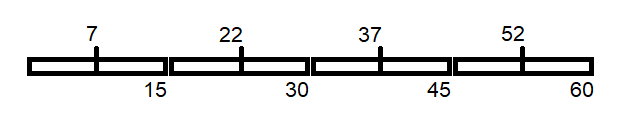
\includegraphics[width=9cm]{sampling-diagram.png}}
\caption{This diagram demonstrates how records were selected to generate 15-minute sampled datasets from the NIST weather station by selecting only 4 records at the 7th, 22nd, 37th, and 52nd minutes. Then to simulate satellite data, these 4 instantaneous records were averaged together to create a single value for the hour.}
\label{fig:sampling-diagram}
\end{figure}

\section{Results}
\label{section:results}

\subsection{Analysis of NIST Ground Array}
The energy yield, POA, and clipping losses for each of the 15 SolarFarmer predictions for the NIST ground array are shown in Table~\ref{table:results-summary}. A plot of the energy yield in Fig.~\ref{fig:NIST-energy-yield} shows the time-averaged, instantaneous, and simulated satellite results. The 1-minute time-averaged measurements correctly account for rapid ramp rates in the solar resource when predicting energy yield, POA, and clipping loss. However, as the time-averaging interval increases to hourly, the energy yield is over-predicted by 2.7\% and the clipping loss is under-predicted by 1.1\% relative to the 1-minute measurements.

\begin{table}[htbp]
\caption{Summary of SolarFarmer Results for NIST Ground Array}
\begin{center}
\begin{tabular}{|c|c|c|c|c|}
\hline
\textbf{Dataset} & \textbf{\textit{Interval}}& \textbf{\textit{Energy Yield}}& \textbf{\textit{POA}}& \textbf{\textit{Clipping}} \\
                 & \textit{minutes}& \textit{kWh/kWp}& \textit{kWh/m\textsuperscript{2}}& \textbf{\textit{Loss}} \\
\hline
             &  1& 1286.3& 1667.4& -4.6\% \\
             &  5& 1298.3& 1669.2& -4.2\% \\
time-averaged& 15& 1308.7& 1671  & -3.9\% \\
             & 30& 1314.8& 1672  & -3.8\% \\
             & 60& 1320.8& 1673.5& -3.5\% \\
\hline
             &  1& 1286.3& 1667.4& -4.6\% \\
             &  5& 1285.9& 1667.7& -4.6\% \\
instantaneous& 15& 1285.4& 1668.2& -4.6\% \\
             & 30& 1285.6& 1665.1& -4.5\% \\
             & 60& 1284  & 1663.1& -4.5\% \\
\hline
             &  1& 1320.8& 1673.5& -3.5\% \\
simulated-   &  5& 1319.3& 1673.6& -3.6\% \\
satellite    & 15& 1315  & 1673.8& -3.7\% \\
             & 30& 1304.9& 1669  & -3.9\% \\
             & 60& 1284  & 1663.1& -4.5\% \\
\hline
\end{tabular}
\label{table:results-summary}
\end{center}
\end{table}

The instantaneous results are also shown in Fig.~\ref{fig:NIST-energy-yield}. The 1-minute results are identical to the 1-minute time-averaged, because the measurement resolution is every minute. As input data is sampled at lower frequency (longer sampling rates), random errors occur in the input data and cancel out the modeling error.

The simulated satellite results are also shown in Fig.~\ref{fig:NIST-energy-yield}. The 1-minute results are identical to the 60-minute time-averaged, because they both show 1-minute measurements averaged hourly. As input data is sampled at increasing frequency (shorter sampling rates), the modeling errors become more apparent. Because all of the simulated satellite input is hourly, this trend is similar but opposite to the increase in modeling errors observed in time-averaged input as the interval is increased. The inflection point seems to be around 30-minutes. At sampling times longer than 30-minutes, random errors occur in the input data and cancel out the modeling error, similar to observations of the instantaneous input. However, we observe that even for input data sampled every 30-minutes, similar to the sampling rate of NSRDB TMY3 files, there is still non-zero modeling error.

\begin{figure}[htbp]
\centerline{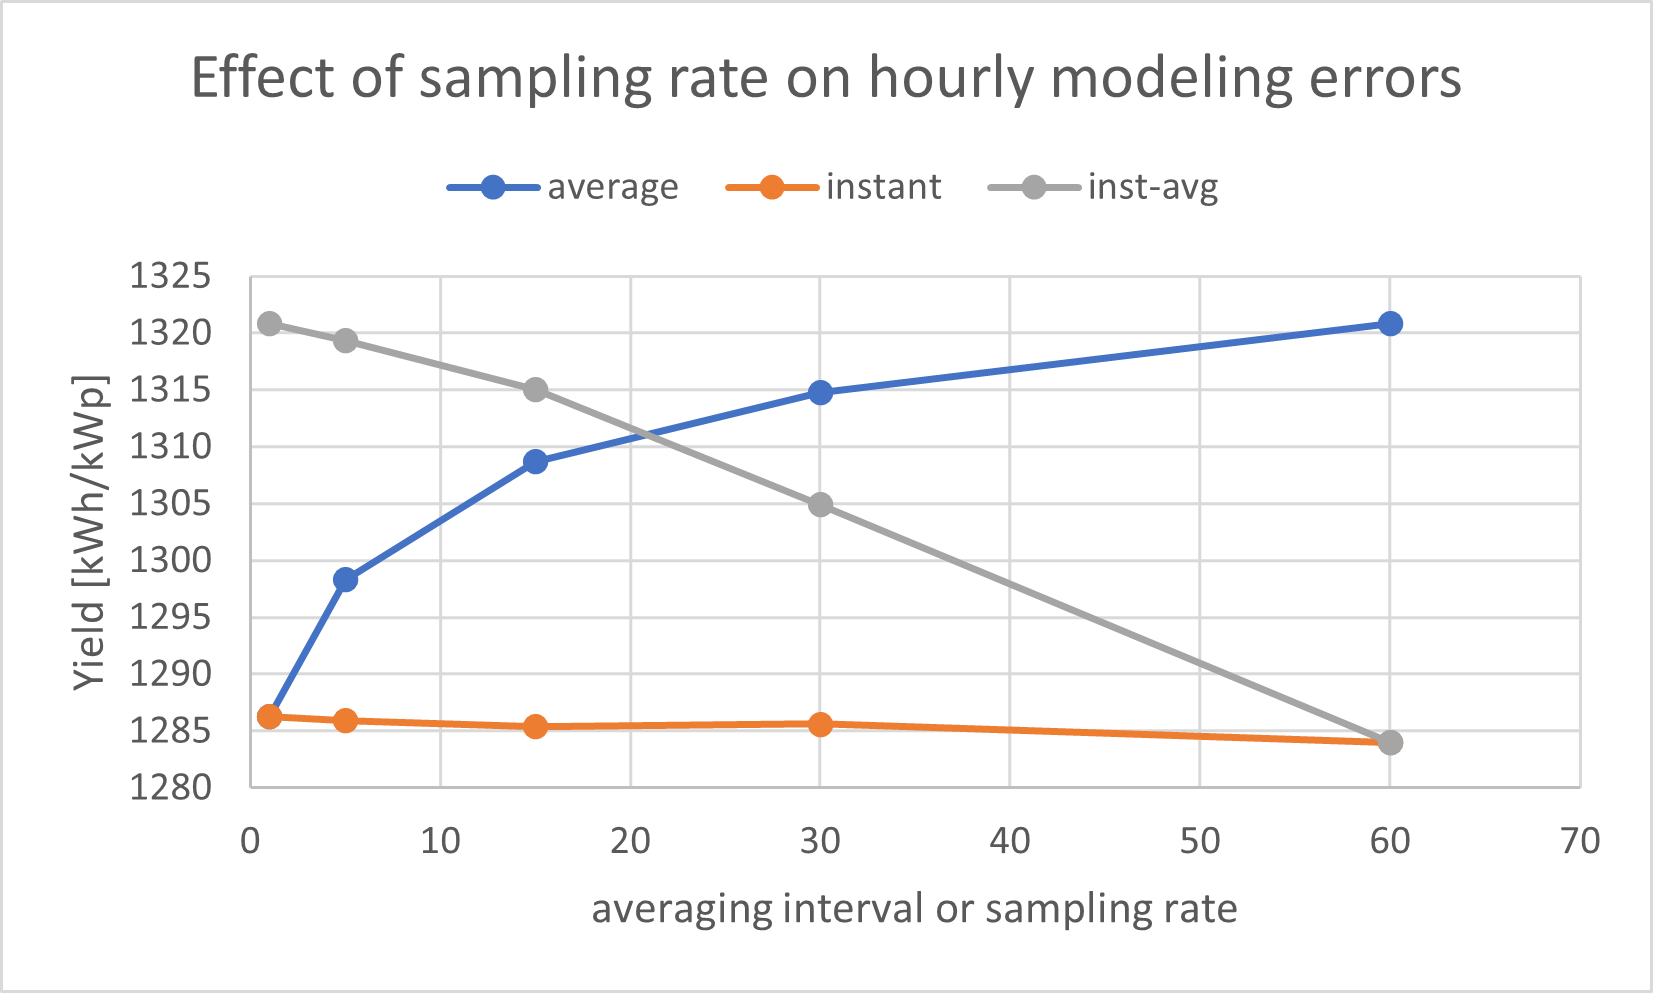
\includegraphics[width=9cm]{NIST_energy_yield.png}}
\caption{Energy yield for all 3 datasets shows over-prediction relative to 1-minute if time-averaged to 60-minutes. Simulated satellite (inst-avg) has non-zero errors at 30-minute sampling rates and increasing errors for shorter sampling rates. Instantaneous has random errors that cancel out.}
\label{fig:NIST-energy-yield}
\end{figure}

\begin{figure}[htbp]
\centerline{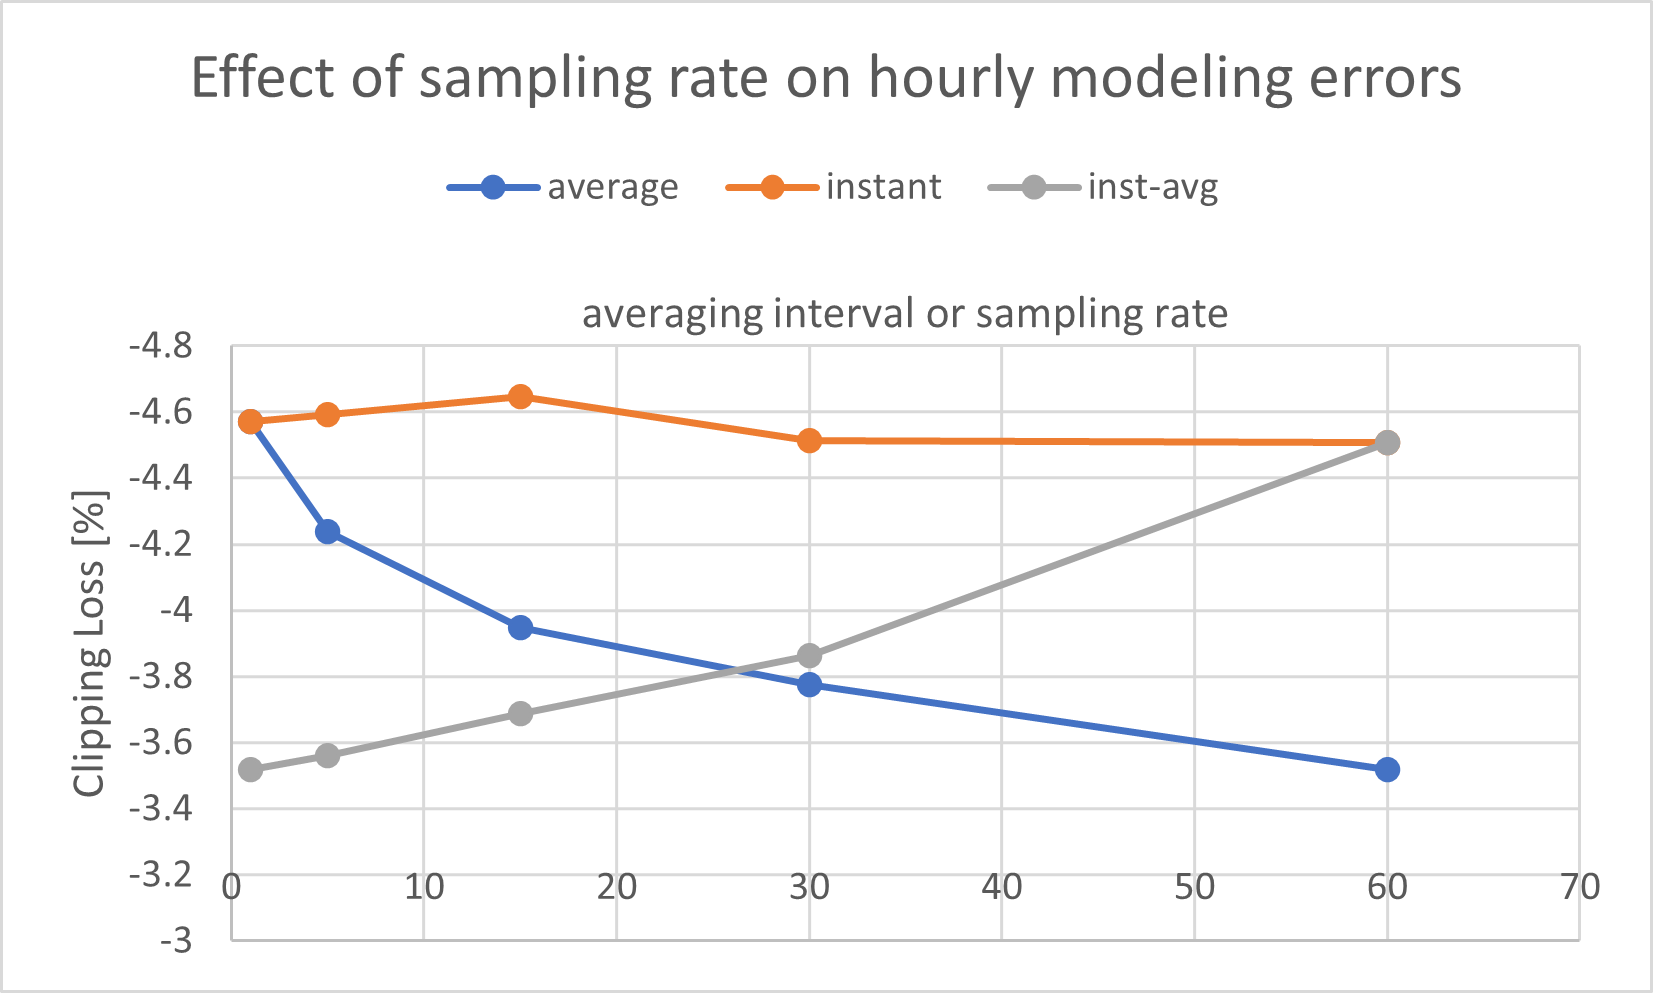
\includegraphics[width=9cm]{NIST_clipping_loss.png}}
\caption{Clipping losses for all 3 datasets shows under-prediction relative to 1-minute if time-averaged to 60-minutes. Simulated satellite (inst-avg) has non-zero errors at 30-minute sampling rate and increasing errors for shorter sampling rates. Instantaneous has random errors that cancel out.}
\label{fig:NIST-clipping-loss}
\end{figure}

\begin{figure}[htbp]
\centerline{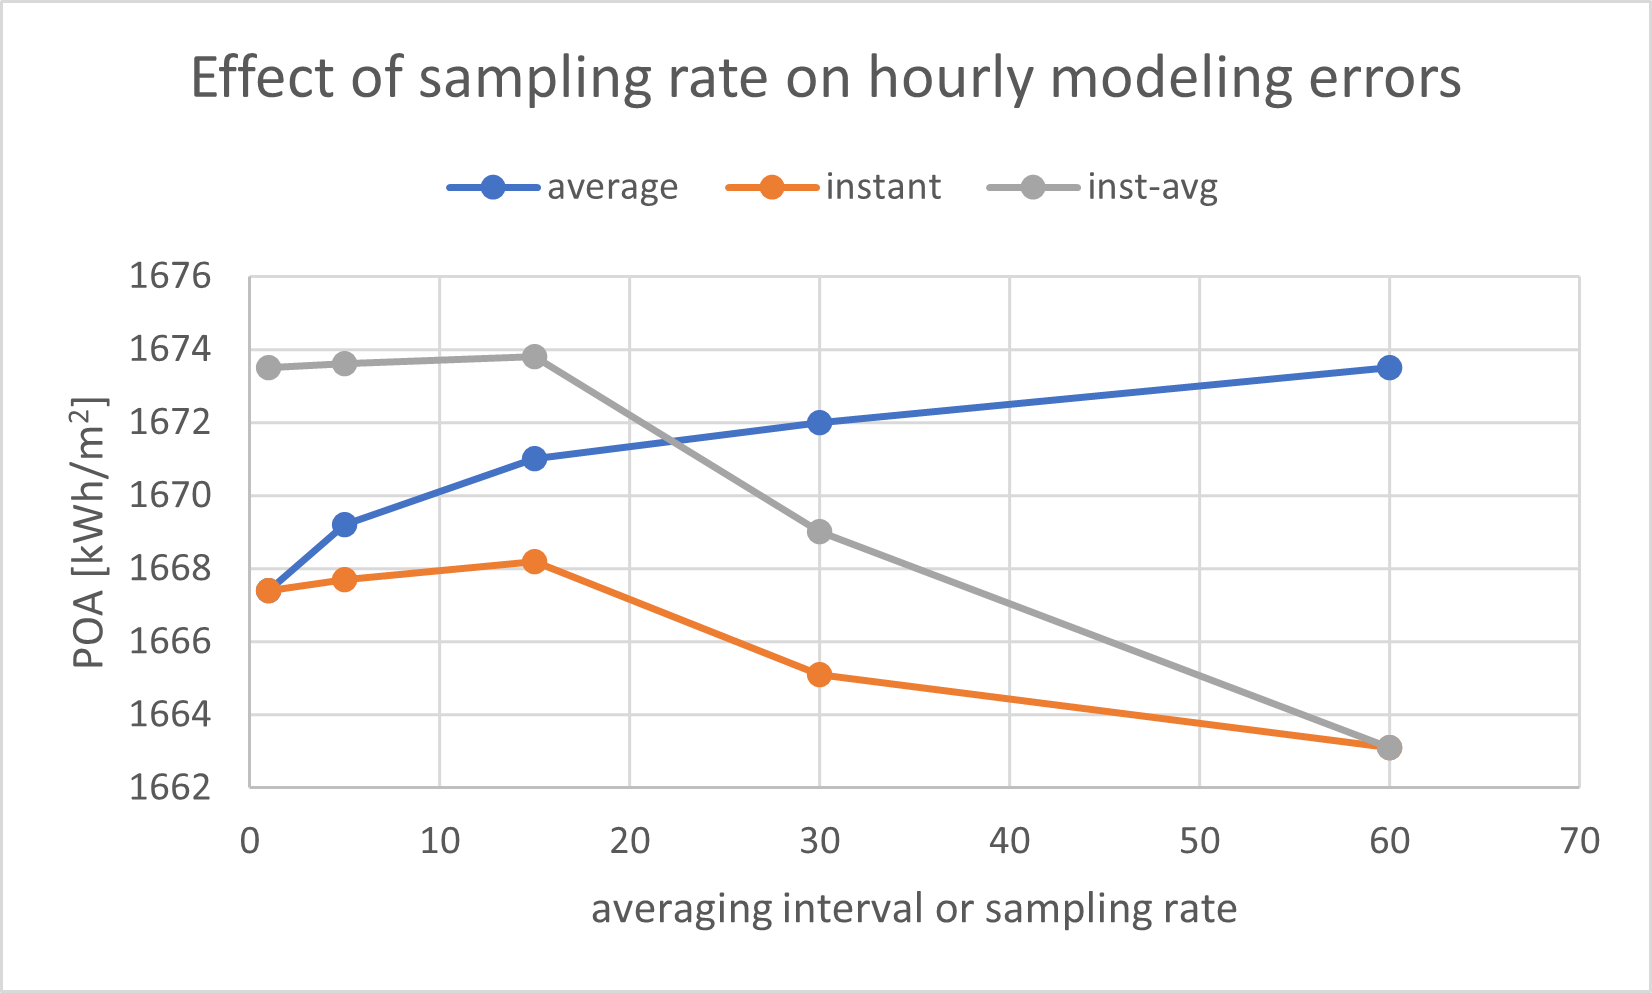
\includegraphics[width=9cm]{NIST_POA.png}}
\caption{POA for all 3 datasets shows significantly smaller errors compared to energy yield, implying that clipping errors dominate modeling errors due to hourly input.}
\label{fig:NIST-POA}
\end{figure}

Clipping losses for all 3 datasets are shown in Fig.~\ref{fig:NIST-clipping-loss}. Clipping losses are the percentage of AC power that is lost due to clipping. Do not compare modeling error between simulations based on clipping loss, because the delta in clipping losses is not equal to the modeling error! For example, the modeling error due to time-averaged hourly input was 2.7\% while the clipping losses only changed by 1.1\%. The modeling error due to hourly inputs is only defined by the change in AC power relative to 1-minute input. However, the clipping loss is useful in determining that clipping errors are the cause of the over-prediction in energy yield.

The POA, shown Fig.~\ref{fig:NIST-POA}, is also over-predicted when using hourly time-averaged inputs relative to 1-minute. However, the POA error is only 0.4\%, significantly less than the modeling error in energy yield. Therefore, we observe that clipping errors dominate the hourly modeling error.

\subsection{Analysis of Generic Array with SURFRAD}
Annual AC energy predicted for the generic array with pvlib python for each of the 15 datasets for each of the 7 SURFRAD stations are shown in Fig.~\ref{fig:bon2010}, \ref{fig:dra2011}, \ref{fig:fpk2009}, \ref{fig:gwn2012}, \ref{fig:psu2010}, \ref{fig:sxf2009}, \& \ref{fig:tbl2010}. The annual AC energy at 1-minute and hourly averages as well as the modeling errors for hourly averaged input and for satellite simulated with 30-minute sampling rate both relative to 1-minute are summarized in Table  \ref{table:SURFRAD-summary} for the first year.

\begin{table}[htbp]
\caption{Summary of Modeling Errors for SURFRAD Generic Arrays with pvlib python}
\begin{center}
\begin{tabular}{|c|c|c|c|c|c|}
\hline
\textbf{Station-}& \textbf{\textit{Egrid}}& \textbf{\textit{Egrid}}& \textbf{\textit{Model}}& \textbf{\textit{Egrid}}& \textbf{\textit{Model}} \\
              \textbf{Year}& \textbf{\textit{1m-inst}}& \textbf{\textit{60m-avg}}& \textbf{\textit{Error}}& \textbf{\textit{30m-sat}}& \textbf{\textit{Error}} \\
                 & \textit{MWh}& \textit{MWh}& \textit{60m-avg}& \textit{MWh}& \textit{30m-sat} \\
\hline
bon-2010& 589& 599& 1.7\%&594& 0.9\% \\
dra-2011& 795& 802& 0.8\%&795& 0.03\% \\
fpk-2009& 576& 588& 2.2\%&584& 1.3\% \\
gwn-2012& 621& 629& 1.3\%&623& 0.3\% \\
psu-2010& 518& 528& 2.0\%&522& 0.7\% \\
sxf-2009& 559& 568& 1.6\%&564& 0.8\% \\
tbl-2012& 632& 648& 2.6\%&643& 1.7\% \\
\hline
\end{tabular}
\label{table:SURFRAD-summary}
\end{center}
\end{table}

The largest modeling errors are at Boulder, CO, for both hourly averaged and simulated satellite at 30-minute sampling rate. Desert Rock, NV, which as the highest annual AC energy output has the lowest modeling errors, but they are still non-zero. Goodwin Creek, MS, has the second lowest modeling errors yet its annual AC production is similar to Boulder, CO. The lowest annual AC output is at Penn State, PA, and it has the 3rd largest modeling error. On average error of the simulated satellite data sampled at 30-minutes, is about half of error of the hourly averages compared to the 1-minute data.

\begin{figure}[htbp]
\centerline{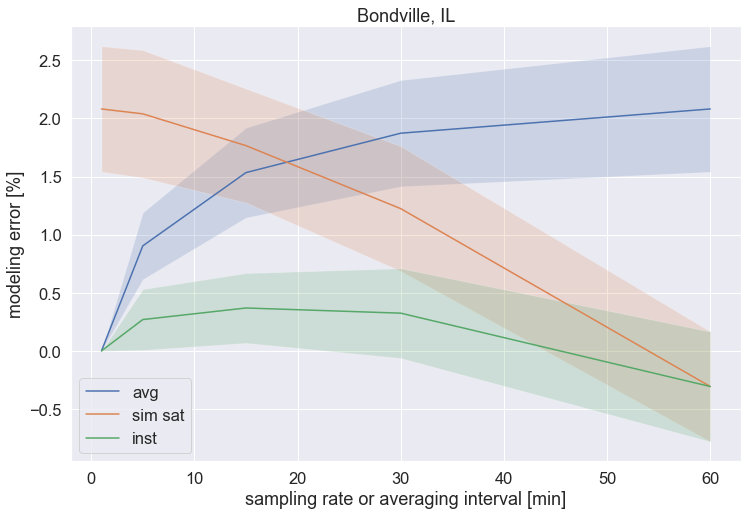
\includegraphics[width=9cm]{analysis/bon_all.png}}
\caption{Annual AC energy modeling error at Bondville, IL. The solid lines and shaded areas show the average and 1-$\sigma$. Time-averaged input (blue) increases with longer averaging interval, simulated satellite (red) decreases with slower sampling rate, while instantaneous (green) is relatively unchanged.}
\label{fig:bon2010}
\end{figure}

\begin{figure}[htbp]
\centerline{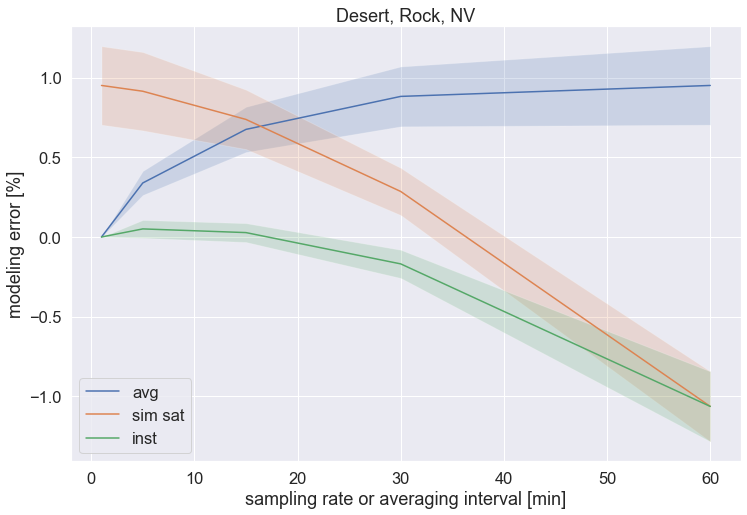
\includegraphics[width=9cm]{analysis/dra_all.png}}
\caption{Annual AC energy modeling error at Desert Rock, NV. The solid lines and shaded areas show the average and 1-$\sigma$. Desert Rock had the highest output and the lowest modeling error of the 7 SURFRAD sites presumably due to its high irradiance and clear skies.}
\label{fig:dra2011}
\end{figure}

\begin{figure}[htbp]
\centerline{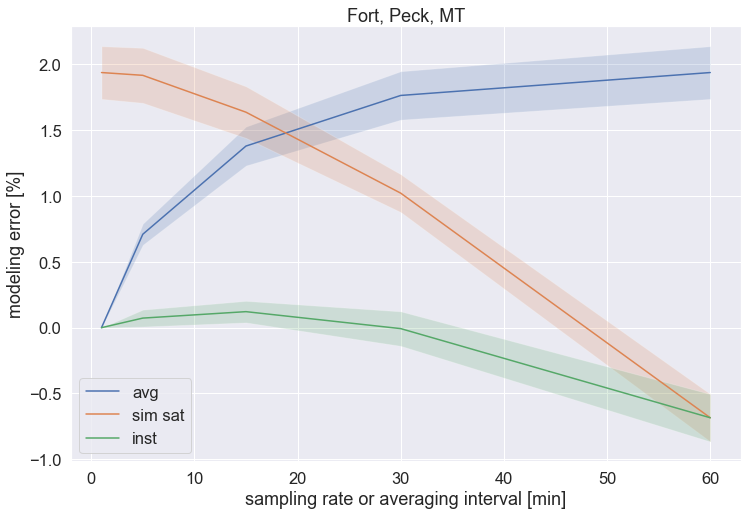
\includegraphics[width=9cm]{analysis/fpk_all.png}}
\caption{Annual AC energy modeling error at Fort Peck, MT. The solid lines and shaded areas show the average and 1-$\sigma$. Time-averaged input (blue) increases with longer averaging interval, simulated satellite (red) decreases with slower sampling rate, while instantaneous (green) is relatively unchanged.}
\label{fig:fpk2009}
\end{figure}

\begin{figure}[htbp]
\centerline{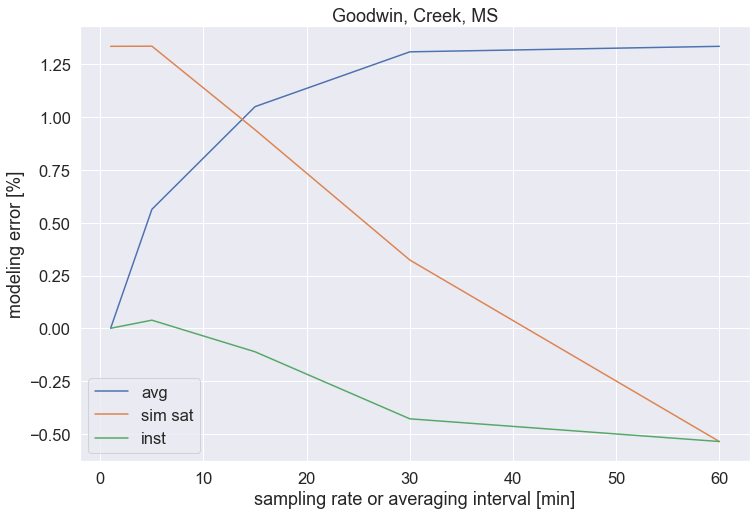
\includegraphics[width=9cm]{analysis/gwn_all.png}}
\caption{Annual AC energy modeling error at Goodwin Creek, MS. There was only one year with sufficient data quality. Time-averaged input (blue) increases with longer averaging interval, simulated satellite (red) decreases with slower sampling rate, while instantaneous (green) is relatively unchanged.}
\label{fig:gwn2012}
\end{figure}

\begin{figure}[htbp]
\centerline{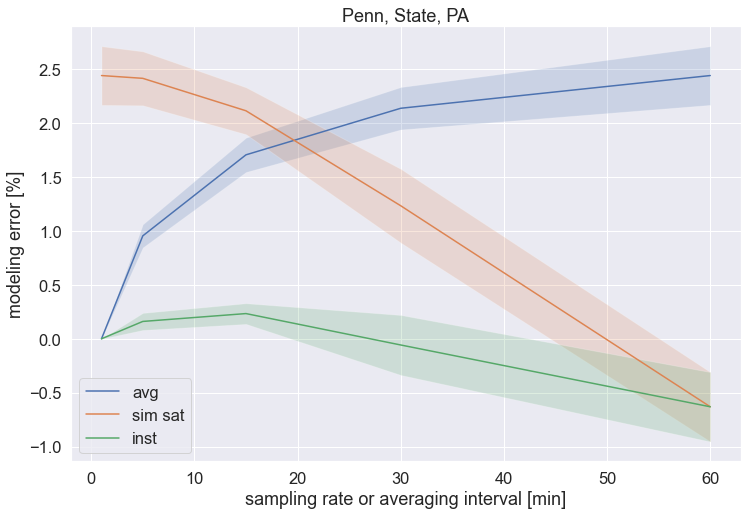
\includegraphics[width=9cm]{analysis/psu_all.png}}
\caption{Annual AC energy modeling error at Penn State, PA. The solid lines and shaded areas show the average and 1-$\sigma$. Time-averaged input (blue) increases with longer averaging interval, simulated satellite (red) decreases with slower sampling rate, while instantaneous (green) is relatively unchanged.}
\label{fig:psu2010}
\end{figure}

\begin{figure}[htbp]
\centerline{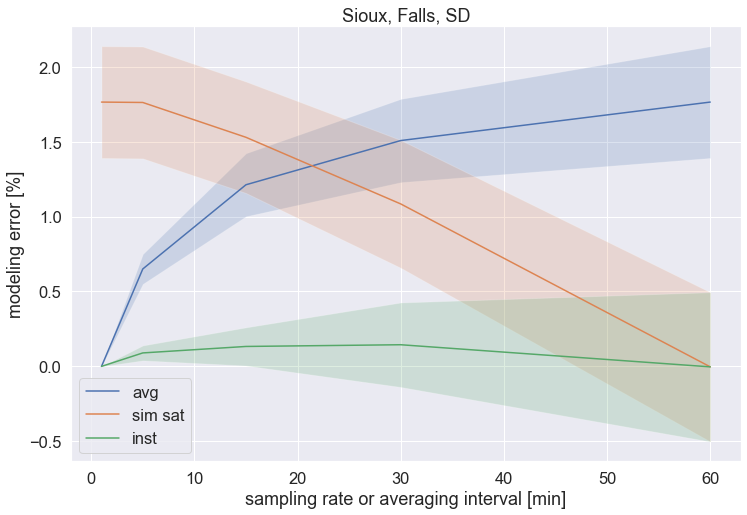
\includegraphics[width=9cm]{analysis/sxf_all.png}}
\caption{Annual AC energy modeling error at Sioux Falls, SD. The solid lines and shaded areas show the average and 1-$\sigma$. Time-averaged input (blue) increases with longer averaging interval, simulated satellite (red) decreases with slower sampling rate, while instantaneous (green) is relatively unchanged.}
\label{fig:sxf2009}
\end{figure}

\begin{figure}[htbp]
\centerline{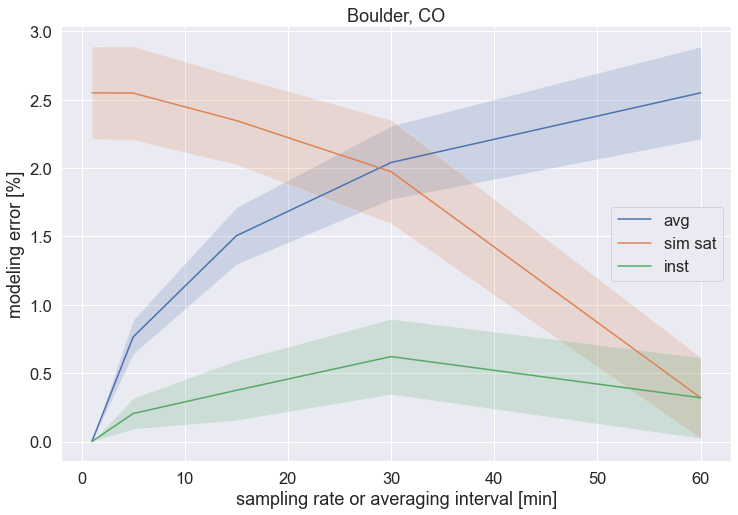
\includegraphics[width=9cm]{analysis/tbl_all.png}}
\caption{Annual AC energy modeling error at Boulder, CO. The solid lines and shaded areas show the average and 1-$\sigma$. Time-averaged input (blue) increases with longer averaging interval, simulated satellite (red) decreases with slower sampling rate, while instantaneous (green) is relatively unchanged.}
\label{fig:tbl2010}
\end{figure}

\section{Conclusions}
Accurate predictions of energy output are important for decreasing the cost of capital for PV systems, but reports of under-performance for the past few years could damage investor confidence. Modeling errors have been observed when using hourly input data for sites with high solar variability and DC/AC greater than one. However, satellite data is averaged from coarsely sampled instantaneous measurements with random hourly errors that appear to reduce these modeling errors. We examined the effect of sampling rate on modeling errors by simulating satellite data from high frequency ground measurements at the NIST ground array and predicting energy output using SolarFarmer. We repeated this analysis using inputs from the 7 SURFRAD stations and predicted energy output using pvlib python. We observed modeling errors for simulated satellite input sampled every 30-minutes or shorter, and the errors increased for shorter sampling rates. We also observed that clipping errors dominated over other sources like POA except at sites with high annual energy output. Therefore, we recommend applying an hourly modeling correction whenever hourly input is used. On average we found this correction can be halved when using satellite data.

\bibliographystyle{IEEEtran}
% argument is your BibTeX string definitions and bibliography database(s)
\bibliography{IEEEabrv,bibliography}
%\balance

\end{document}
